\documentclass{beamer}
\mode<presentation>
\usepackage{amsmath}
\usepackage{amssymb}
%\usepackage{advdate}
\usepackage{adjustbox}
\usepackage{subcaption}
\usepackage{enumitem}
\usepackage{multicol}
\usepackage{mathtools}
\usepackage{listings}
\usepackage{float}
\usepackage{graphicx}
\usepackage{url}
\usepackage{lmodern}
\usepackage[utf8]{inputenc}
\usepackage{xcolor}
\def\UrlBreaks{\do\/\do-}
\usetheme{Boadilla}
\usecolortheme{lily}
\setbeamertemplate{footline}
{
  \leavevmode%
  \hbox{%
  \begin{beamercolorbox}[wd=\paperwidth,ht=2.25ex,dp=1ex,right]{author in head/foot}%
    \insertframenumber{} / \inserttotalframenumber\hspace*{2ex} 
  \end{beamercolorbox}}%
  \vskip0pt%
}
\setbeamertemplate{navigation symbols}{}

\providecommand{\nCr}[2]{\,^{#1}C_{#2}} % nCr
\providecommand{\nPr}[2]{\,^{#1}P_{#2}} % nPr
\providecommand{\mbf}{\mathbf}
\providecommand{\pr}[1]{\ensuremath{\Pr\left(#1\right)}}
\providecommand{\qfunc}[1]{\ensuremath{Q\left(#1\right)}}
\providecommand{\sbrak}[1]{\ensuremath{{}\left[#1\right]}}
\providecommand{\lsbrak}[1]{\ensuremath{{}\left[#1\right.}}
\providecommand{\rsbrak}[1]{\ensuremath{{}\left.#1\right]}}
\providecommand{\brak}[1]{\ensuremath{\left(#1\right)}}
\providecommand{\lbrak}[1]{\ensuremath{\left(#1\right.}}
\providecommand{\rbrak}[1]{\ensuremath{\left.#1\right)}}
\providecommand{\cbrak}[1]{\ensuremath{\left\{#1\right\}}}
\providecommand{\lcbrak}[1]{\ensuremath{\left\{#1\right.}}
\providecommand{\rcbrak}[1]{\ensuremath{\left.#1\right\}}}
\theoremstyle{remark}
\newtheorem{rem}{Remark}
\newcommand{\sgn}{\mathop{\mathrm{sgn}}}
\providecommand{\abs}[1]{\left\vert#1\right\vert}
\providecommand{\res}[1]{\Res\displaylimits_{#1}} 
\providecommand{\norm}[1]{\lVert#1\rVert}
\providecommand{\mtx}[1]{\mathbf{#1}}
\providecommand{\mean}[1]{E\left[ #1 \right]}
\providecommand{\fourier}{\overset{\mathcal{F}}{ \rightleftharpoons}}
%\providecommand{\hilbert}{\overset{\mathcal{H}}{ \rightleftharpoons}}
\providecommand{\system}{\overset{\mathcal{H}}{ \longleftrightarrow}}
	%\newcommand{\solution}[2]{\textbf{Solution:}{#1}}
%\newcommand{\solution}{\noindent \textbf{Solution: }}
\providecommand{\dec}[2]{\ensuremath{\overset{#1}{\underset{#2}{\gtrless}}}}
\newcommand{\myvec}[1]{\ensuremath{\begin{pmatrix}#1\end{pmatrix}}}
\let\vec\mathbf

\lstset{
frame=single, 
breaklines=true,
keepspaces=true,
columns=fullflexible
}
\numberwithin{equation}{section}

\title{\textcolor{red}{\underline{\textbf{Area Under Graph}}}}
\author{\textcolor{red}{\textbf{EE24BTECH11048-NITHIN.K}}}

\date{\textcolor{red}{\today}}
\begin{document}

\begin{frame}
	\titlepage
\end{frame}

\section*{Outline}
\begin{frame}
	\frametitle{\underline{\textbf{Table of Contents}}}
	\tableofcontents
\end{frame}

\section{Problem}
\begin{frame}
	\frametitle{\underline{Problem Statement}}
	\textbf{Area lying in the first quadrant and bounded by the circle $x^2 + y^2 = 4$ and the lines $x = 0$ and $x = 2$ is?}
\end{frame}

\section{Solution}
\begin{frame}
	\frametitle{\underline{Solution}}
		\begin{table}[H]
			\centering
			\resizebox{\textwidth}{!}{
				\begin{center}
    \begin{tabular}{|c|c|c|} 
        \hline
            \textbf{FUNCTION} & \textbf{FORMULA} \\
        \hline
            $g\brak{x}$ & $\vec{x^TVx}+\vec{2u^Tx}+f=0$ \\
        \hline
	    The points of intersection & $ L: \vec{x} = \vec{h} + \kappa\vec{m}, \kappa \in \mathbb{R} $ \\ of the line L with the conic & $\kappa_i = \frac{1}{\vec{m^TVm}}\brak{\vec{-m^T\brak{Vh+u}} \pm \sqrt{\sbrak{\vec{m^T\brak{Vh+u}}^2} - g(\vec{h})\brak{\vec{m^TVm}}}} $ \\ section as above are \\ given by $ \vec{x}_i = \vec{h} + \kappa_i\vec{m} $ \\
        \hline
    \end{tabular}
\end{center}

			}
			\caption{Variables Used}
		\end{table}
\end{frame}

\begin{frame}
	\frametitle{Solution}
	\small
	On comparing $g\brak{x}$ and $x^2 + y^2 - 4 = 0$ the parameters of the circle are
	\begin{align}
		\vec{V} = \myvec{ 1 & 0 \\
		0 & 1 } \\
		\vec{u} = \myvec{0 \\
		0 } \\
		f = -4
	\end{align}
	The area bounded by $x=0$, $x=2$ and the circle in the first quadrant is
	\begin{align}
		\int_{0}^{2}\sqrt{4 - x^2} dx
	\end{align}
	for indefinite integration of above form we get
	\begin{align}
		\int\sqrt{4 - x^2} dx = 2\sin^{-1}\frac{x}{2} + x\sqrt{4 - x^2} + c \\
		\int_{0}^{2}\sqrt{4 - x^2} dx = \pi
	\end{align}
	Hence the enclosed area is $\pi$ square units
\end{frame}

\section{Codes}
\begin{frame}[fragile]
	\frametitle{\underline{C Code for Calculating Area}}
	\begin{lstlisting}[language=C]
	#include <stdio.h>
	#include <math.h>
	double area(double lower_limit, double upper_limit){
		double sum=0 ;
		for ( double i = lower_limit; i<=upper_limit; i+=1e-7 ){
			sum += sqrt(4-(i*i))*1e-7;
		}
		return sum ;
	}
	\end{lstlisting}
\end{frame}

\begin{frame}[fragile]
	\frametitle{\underline{Python Code using shared library}}
	\begin{lstlisting}[language=Python]
	import ctypes
	lib = ctypes.CDLL('./integration.so')
	lib.area.argtypes = [ctypes.c_double, ctypes.c_double]
	lib.area.restype = ctypes.c_double
	print("Area enclosed",lib.area(0,2))
	\end{lstlisting}
\end{frame}

\begin{frame}[fragile]
	\frametitle{\underline{Python Code for Plotting}}
	\begin{lstlisting}[language=Python]
	import sys
	sys.path.insert(0, '/home/nithink/matgeo/codes/CoordGeo')
	import numpy as np
	import matplotlib.pyplot as plt
	from numpy import linalg as LA
	
	# local imports
	from line.funcs import *
	from triangle.funcs import *
	from conics.funcs import *

	r = 2
	V = np.eye(2)
	u = np.array(([0, 0])).reshape(-1, 1)
	f = -4
	\end{lstlisting}
\end{frame}
\begin{frame}[fragile]
	\frametitle{Python Code for Plotting}
	\begin{lstlisting}[language=Python]
	# Generating circle
	x_circ = circ_gen(-u, r)
	
	n1 = np.array(([1, 0])).reshape(-1,1) 
	c1 = 0
	n2 = np.array(([1, 0])).reshape(-1,1)
	c2 = 2
	k1 = -4
	k2 = 4
	
	#Generating Lines
	x_A = line_norm(n1,c1,k1,k2)
	x_B = line_norm(n2,c2,k1,k2)
	\end{lstlisting}
\end{frame}
\begin{frame}[fragile]
	\frametitle{Python Code for Plotting}
	\begin{lstlisting}[language=Python]
	# Plotting all lines and circles
	plt.plot(x_circ[0, :], x_circ[1, :], label='$Circle$')
	plt.plot(x_A[0,:],x_A[1,:],label='$x = 0$')
	plt.plot(x_B[0,:],x_B[1,:],label='$x = 2$')

	# Adjusting axis spines
	ax = plt.gca()
	ax.spines['top'].set_color('none')
	ax.spines['left'].set_position('zero')
	ax.spines['right'].set_color('none')
	ax.spines['bottom'].set_position('zero')

	# Define the space
	x = np.linspace(0,2,100)
	y_circle = np.sqrt(4-x**2)
	\end{lstlisting}
\end{frame}
\begin{frame}[fragile]
	\frametitle{Python Code for Plotting}
        \begin{lstlisting}[language=Python]
	# Fill the area between the lines and the circle
	plt.fill_between(x,0, y_circle, color='red', alpha=0.5, label='Shaded Region')

	# Labels and title
	plt.xlabel('x')
	plt.ylabel('y')
	
	# Final plot settings
	plt.legend(loc='upper right')
	plt.axis('equal')
	
	#Display the Plot
	plt.show()
	\end{lstlisting}
\end{frame}

\begin{frame}
	\frametitle{\underline{Diagram}}
	\begin{figure}[H]
		\centering
		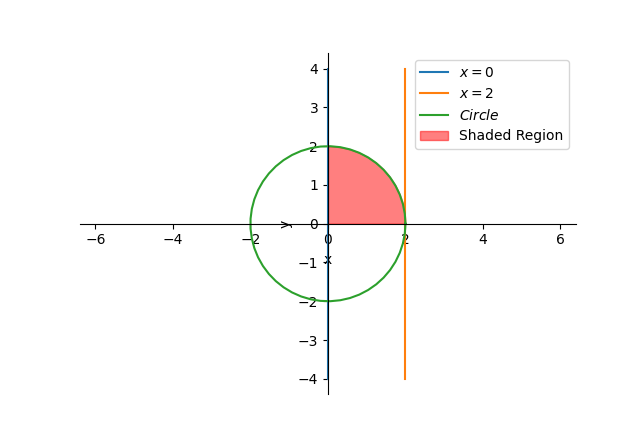
\includegraphics[width=0.7\linewidth]{figs/Figure_1.png}
		\caption{Enclosed Area}
	\end{figure}
\end{frame}
\end{document}
